\section{Introduction and Motivation}



% Intro
% * Hva skjer
% * Hvorfor er dette et problem
% * Kan vi gjøre noe med det?
% * Hva gjør vi for å komme nærmere en løsning
% * Hva har vi fått til
% * Noe ekstra dette kan brukes til




% Hva skjer
As we are standing on the doorstep of the ages of Dark Silicon,
increased energy efficiency is a key factor to allow more performance.
\autoref{fig:cpuperformace} tells us how single-threaded performance
almost halted as we hit the power wall. Because of the end of Dennard
scaling, further shrinking of the transistor did not shrink the power
dissipated by each one of them. This leads to a rapid increase in
power denisty, and if the industry continues cramming more logic to
single threaded performace, wattage per area would be too high
for common cooling techniques.

Another problem arising as feature size decreases is that the
static power drain seems to be a more and more significant part of energy
consumption, and thus also heat. As transistors went below below 0.1 micron,
static power drain started to pose a real challenge
\cite{kim2003leakage,martin2002combined}.  \autoref{fig:staticdynamic} shows how
power flows through a set of transistors. When the network toggles, a small
charge is let from VCC to C or from C to GND, also, as the transistors are
becomming smaller some current leaks over it as if it was an ordinary resistor
\cite{wolf}. As feature size becomes small enough, simply powering the chip
without toggeling bits generates a significant amount of heat.


\begin{figure}
    \centering
    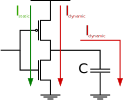
\includegraphics[width=0.5\textwidth]{figs/static-dynamic.pdf}
    \caption{Static and dynamic power through a PMOS and NMOS transistor}
    \label{fig:staticdynamic}
\end{figure}



When faster hardware can no longer be created by just adding more
logic, engineers have to look for more energy efficient solutions
in order to keep power density down. Current research consists of
many branches reaching from homogeneous processors to heterogeneous
systems with loads of interconnect.

\begin{figure}
\begin{subfigure}[b]{0.48\textwidth}
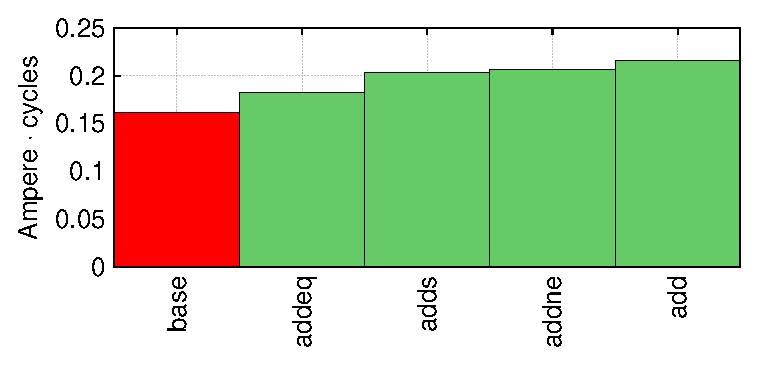
\includegraphics[width=\textwidth]{graph_01_base_cond-0c6.eps}
\caption{Conditional execution (eq is false).}
\end{subfigure}
\begin{subfigure}[b]{0.52\textwidth}
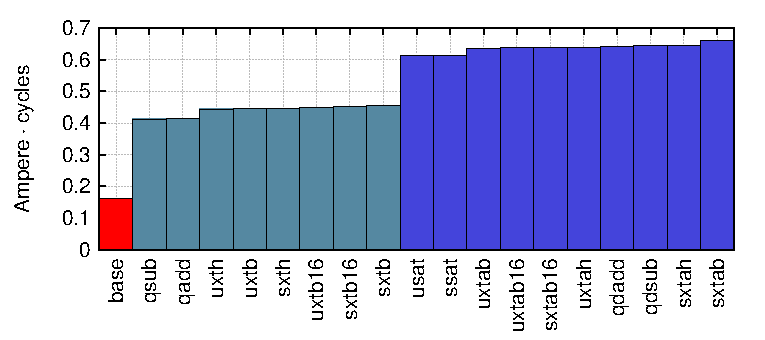
\includegraphics[width=\textwidth]{graph_023_base_quad_saturate_extend-0c6.eps}
\caption{Non-multiply multi-cycle instructions.}
\end{subfigure}
\caption{Figures from \cite{rundehvatum2013exploring} showing the results of measuring the
current drain through the CPU core while running isolated instructions in a loop.}
\end{figure}

\cite{wolf} talks about static vs. dynamic as well as energy vs. power in chapter 3.6.

Static vs. dynamic power, what it means for further shrinking, dark silicon, powering
the entire chip vs. lower freq.

emphasize energy efficiancy over pure performce 

\begin{figure}
    \centering
    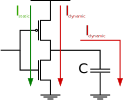
\includegraphics[width=0.5\textwidth]{figs/static-dynamic.pdf}
    \caption{Static and dynamic power}
    \label{fig:staticdynamic}
\end{figure}

In \autoref{fig:staticdynamic} we see how the power drawn from switching is charged up and then released
through the capacitor and the transistor, while the static power leaks through the transistor as if
it was a resistor.

